\documentclass[conference]{IEEEtran}
\IEEEoverridecommandlockouts
% The preceding line is only needed to identify funding in the first footnote. If that is unneeded, please comment it out.

\usepackage{cite}
\usepackage{amsmath,amssymb,amsfonts}
\usepackage{algorithmic}
\usepackage{graphicx}
\usepackage{textcomp}
\usepackage{xcolor}
\usepackage{booktabs}
\usepackage{multirow}
\usepackage[caption=false,font=footnotesize]{subfig}
\usepackage{url}
\usepackage{stfloats}

% Float placement optimization to ensure figures stay in their sections and do not dump at the end
\renewcommand{\topfraction}{0.95}
\renewcommand{\bottomfraction}{0.95}
\renewcommand{\textfraction}{0.05}
\renewcommand{\floatpagefraction}{0.85}
\renewcommand{\dbltopfraction}{0.95}
\renewcommand{\dblfloatpagefraction}{0.85}

\def\BibTeX{{\rm B\kern-.05em{\sc i\kern-.025em b}\kern-.08em
    T\kern-.1667em\lower.7ex\hbox{E}\kern-.125emX}}

\begin{document}

\title{A Dual-Tier Aerial Vision Pipeline for Small-Object Detection, Multi-Target Tracking, and Automated Flow Analytics in UAV Surveillance}

\author{\IEEEauthorblockN{Md. Taher Bin Omar Hijbullah}
\IEEEauthorblockA{\textit{Department of Computer Science and Engineering} \\
\textit{AI/ML Research Group}\\
Dhaka, Bangladesh \\
Email: hijbullah119445@gmail.com}
}

\maketitle

\begin{abstract}
The perception of the world in autonomous aerial surveillance with Unmanned Aerial Vehicles (UAVs) requires high precision accuracy to function in critical operational situation with small ground-sample distance, object occlusion and camera ego-motion. The conventional computer vision models used in terrestrial applications face catastrophic recall degradation in the processing of high-altitude drone video feeds because of the data loss phenomenon by downsampling. Besides, the computational complexity of the heavy sliding-window inference algorithms is too heavy to be processed on real-time edge microprocessors of UAVs in real-time without incurring the latency penalty. 

To tackle these basic problems, this paper suggests a framework for aerial computer vision with two phases: on-line edge processing and deep post-flight analysis. Tier-1 (Real-Time Edge Stream) consists of a custom YOLOv8-Medium architecture, ByteTrack multi-object tracking algorithm, and adaptive full-frame polygon boundary logic, and has a real-time bidirectional (In/Out) flow counting rate of 21--25 frames per second (FPS) and persistent ID association rate of 90\%. Tier-2 (High-Altitude Micro-Analytics Stream) was developed by employing Slicing Aided Hyper Inference (SAHI) and by applying overlapping 640x640 pixel grid slicing to ensure high resolution spatial data for small objects. 

The framework is systematically trained and evaluated on the VisDrone 2019 dataset, which has 10 aerial object categories, on an NVIDIA Tesla T4 GPU, achieving a mean Average Precision at IoU 0.50 (mAP@50) of 0.459, Precision of 0.570 and Recall of 0.457 across 50 epochs. The paradigm is proven in the real world with 4K video feeds from the urban environment through a drone and with excellent recall of the smallest pedestrians and vehicles at the most complex aerial angles, it had the potential to become a powerful and practical tool for smart city monitoring and drone surveillance.
\end{abstract}

\begin{IEEEkeywords}
Unmanned Aerial Vehicle (UAV), Aerial Object Detection, VisDrone, Small Object Detection, Slicing Aided Hyper Inference (SAHI), Multi-Object Tracking, ByteTrack, Zone Counting.
\end{IEEEkeywords}

\section{Introduction}
Unmanned Aerial Vehicles (UAVs) are emerging as important tools in public safety, intelligent transportation systems (ITS), disaster management and urban crowd analytics applications \cite{zhu2021detection, akyon2022sahi}. High performance and intelligence are required for the perception onboard an autonomous drone, which should allow it to detect, identify the identity of objects in time, and take them into account in space. There are, however, several fundamental science and engineering challenges to overcome in the transition to the aerial computer vision -- and these are quite different from those seen in ground-based computer vision pipelines:

\begin{enumerate}
    \item \textbf{Extreme scale variation and microscopic targets:} In combination with the varying angles and wide-angle lenses, target objects such as pedestrians, two-wheelers, small cars are only 8x8 to 20x20 pixels in a multi-megapixel frame. Traditional CNNs reshape the input images to a ``canonical'' size (640x640 in this case), discarding fine-grained features of target objects in earlier layers with strided convolution and pooling \cite{akyon2022sahi}.
    \item \textbf{Dense Occlusion and Viewpoint Distortion:} Viewpoints of top-down and high obliquity result in unusual geometric aspect ratio, non-rigid body deformation, and the presence of a significant amount of background clutter; this leads to higher rate of false positive and false negative.
    \item \textbf{Identification switch and re-identification in motion:} High speed of drones and camera pan-tilt-zoom lead to fast optical flow changes often resulting in loss of tracklet or multiple counting in multi-object tracking algorithms of people moving across different zones \cite{zhang2022bytetrack}.
    \item \textbf{Edge Compute Latency vs. Analytic Accuracy Trade-off:} Larger wattages and thermal envelopes are required for real-time scenarios to enable brute-force high-resolution inference, but these edge companions on UAVs (like the NVIDIA Jetson modules) have limited wattages and thermal envelopes.
\end{enumerate}

This is a problem that existing designs cannot avoid, they either weigh so little that they can detect smaller targets, but work at high frame rates (50 fps or greater) or they are very heavy and work at sub-real-time frame rates (5 fps or less).

In this paper, we propose, implement and benchmark a full-fledged Dual-Tier Aerial Vision Pipeline, with low latency deployment at the edge and high density for small object detection. The major merits of this work are:

\begin{itemize}
    \item \textbf{Dual-Capability System Architecture:} We design and build a multi-tiered pipeline: An onboard edge mode customized trained YOLOv8m network and ByteTrack are used to realize real-time tracking (20--25 FPS); An analytical mode is adopted to realize micro-object recovery by implementing Slicing Aided Hyper Inference (SAHI).
    \item \textbf{Dynamic Full-Frame Polygon Counting:} We design a resolution-invariant and full frame perimeter margin boundary algorithm that calculates the trajectory vectors across the boundaries, and provide a non-directional full frame entry/exit counting without any hard tripwire restriction.
    \item \textbf{Convergence Trajectory Benchmark on VisDrone 2019:} Plot the convergence trajectory for the architecture on the official dataset of the VisDrone 2019 competition for 50 epochs and adjust the architecture and discuss the convergence trajectory, class-wise precision-recall curve and normalized confusion matrix.
    \item \textbf{Real-World Validation and Trade-off Analysis:} We test the system on a real drone video showing 4K urban traffic and quantify the data precisely -- how much throughput, recall and tracking stability we can expect to trade off for every one of these.
\end{itemize}

A literature review on the work related to the aerial detection and tracking is provided in Section II. The methodology and mathematical formulation and architecture is outlined in Section III. In Section IV, the experimental setup is described. Results from both a quantitative and qualitative nature are provided in Section V. Section VI provides an analysis of the trade-offs in deploying on the edges, and Section VII wraps up the paper.

\section{Related Work}

\subsection{Object Recognition in Aerial Imagery with UAVs}
Recently, the object detection in the aerial domain has emerged as a hot topic due to the emergence of large-scale datasets such as VisDrone \cite{zhu2021detection}, UAVDT \cite{du2018unmanned}, and DOTA \cite{xia2018dota}. Two-stage detectors, such as Faster R-CNN \cite{ren2015faster} and Cascade R-CNN, have high localization accuracy but high cost, which is not conducive to their application in the limited resource environment. 

The single-stage YOLO detectors \cite{redmon2016you, bochkovskiy2020yolov4, jocher2023ultralytics}, however, have become the standard for aerial applications due to their best performance in terms of inference throughput and localization. Newer models such as YOLOv8 have added anchor-free detection heads to help on a variety of aspect ratios of the bounding boxes, separation of prediction branches and Distribution Focal Loss \cite{li2020generalized} to offer tremendous advantages over the older anchor-based models.

\subsection{Detection of Small Objects by Slicing Mechanisms}
If the aerial images are 4K or 1080p and then down sampled to 640x640, then small objects will be lost forever. To address this issue, Akyon et al. presented a novel method referred to as Slicing Aided Hyper Inference (SAHI) \cite{akyon2022sahi} that does not require retraining extremely high-resolution networks. SAHI divides the main image into overlapped cropped patches, makes local inference and combines the bounding boxes back on the original spatial coordinates using Non-Maximum Suppression (NMS) algorithm. Being able to recall small targets is a very significant advantage in recall but the overlapping forward passes of SAHI seriously compromise throughput, an empirical situation that must be carefully scheduled by architecture.

\subsection{Multi-Object Tracking (MOT) in Aerial Surveillance}
A high sensitivity of the tracking of multiple objects from the air to the velocity fluctuations of the objects and the velocity fluctuations of the camera. Existing techniques like SORT \cite{bewley2016simple} and DeepSORT \cite{wojke2017simple} employ high confidence threshold detection and Kalman filtering, however, they fail to retain targets when they are occluded or not very visible. In the MOT game Zhang et al. ByteTrack \cite{zhang2022bytetrack} proposed a new idea of connecting all the detection boxes, even low confidence boxes, to the corresponding tracklets. Through the similarity of the detection bounding box and the trajectory prediction of the Kalman filter, ByteTrack is able to estimate true objects in the cases of partial occlusion while suppressing background noise and works particularly well on high altitude UAV feeds.

% ----------------- Architecture Overview Diagram -----------------
\begin{figure*}[!t]
\centering
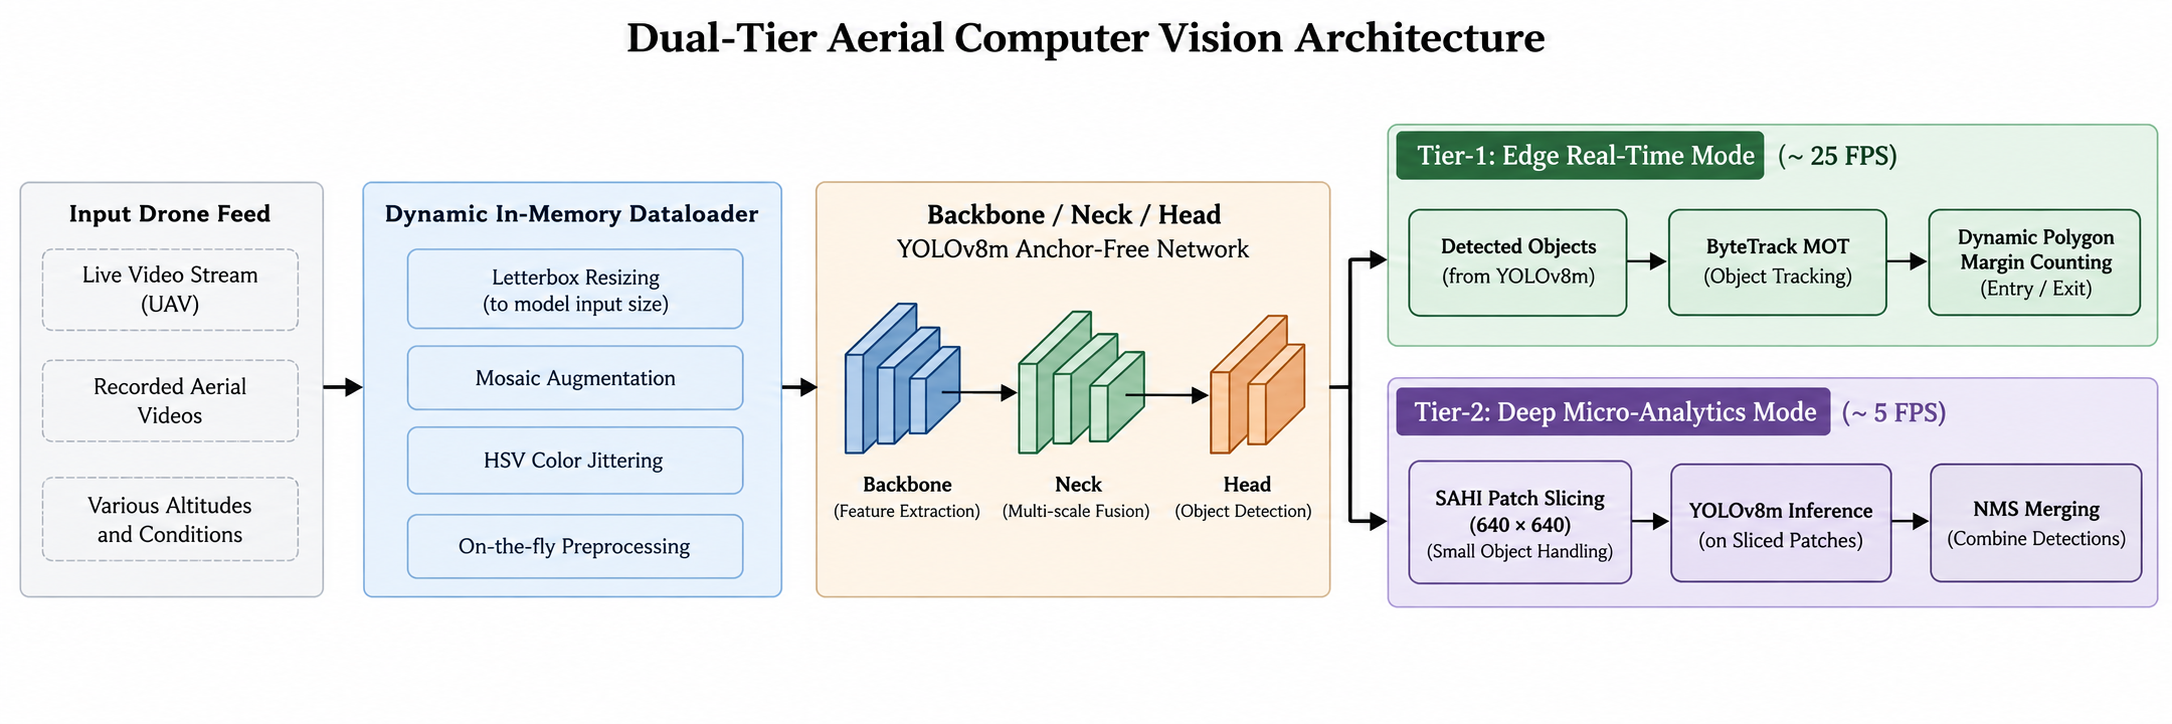
\includegraphics[width=0.98\textwidth]{figures/Architecture.png}
\caption{System architecture of the proposed Dual-Tier Aerial Vision Pipeline, illustrating the concurrent execution paths for real-time edge tracking and post-flight micro-analytics.}
\label{fig:pipeline_arch}
\end{figure*}

\section{Proposed Methodology}

The system architecture proposed in this paper is made up of three synchronized modules: an in-memory dynamic preprocessing engine, a Tier-1 high-speed detection, tracking, and zone-counting stream, and a Tier-2 slicing-aided hyper-inference stream, as depicted in Fig.~\ref{fig:pipeline_arch}.

\subsection{Data Augmentation and Preprocessing}
A huge storage overhead is required for the static pre-generation of augmented datasets and it is not possible to generate a diverse sample. There is an in memory dynamic augmentation pipeline, using the PyTorch dataloader. The following is carried out for each training frame:
\begin{itemize}
    \item \textbf{Adaptive Letterboxing:} Resize with aspect ratio -- with minimum symmetric padding to 640x640 pixels, no geometric elongation of vehicles and pedestrians.
    \item \textbf{Mosaic Augmentation:} In the initial 40 epochs, the network was trained with four randomly selected images and mosaicing them into one synthetic image, forcing the network to learn the objects of different scales of contexts. To ensure stable convergence on native ground truth distributions, the last 10 epochs do not use mosaic (`close\_mosaic=10').
    \item \textbf{HSV Photometric Jitter:} Modulation of hue, saturation and exposure value to manage very bright sunlight and shadow in aerial imaging.
\end{itemize}

\subsection{Object Detection Formulation}
The backbone used is a YOLOv8-Medium (YOLOv8m) to create an instance of the core detector. Their architecture is a feature extractor, CSPDarknet ($C2f$), splits and concatenates the flow of gradients of the features. To represent both large scale spatial field and the small scale spatial field, we use a path-aggregation Feature Pyramid Network (PAN-FPN) that has multi-scale representation at multiple feature strides.

The loss function is a combination of Classification Loss, Bounding Box Regression Loss and Distribution Focal Loss:
\begin{equation}
\mathcal{L}_{total} = \lambda_1 \mathcal{L}_{cls} + \lambda_2 \mathcal{L}_{box} + \lambda_3 \mathcal{L}_{dfl}
\label{eq:total_loss}
\end{equation}

In the case of bounding box regression, Complete Intersection over Union (CIoU) is used to take into consideration the overlap area, central point distance and aspect ratio:
\begin{equation}
\mathcal{L}_{box} = 1 - \text{IoU} + \frac{\rho^2(b, b^{gt})}{c^2} + \alpha v
\label{eq:ciou}
\end{equation}
where $\rho(b, b^{gt})$ represents the Euclidean distance between predicted and ground-truth box centroids, $c$ is the diagonal length of the smallest enclosing box, and $\alpha v$ quantifies aspect-ratio consistency.

The Distribution Focal Loss represents the distribution of the boundaries of the bounding box in the form of continuous probability functions instead of Dirac delta functions, which considerably improves the localization accuracy of ambiguous and occlusion aerial boundaries:
\begin{equation}
\mathcal{L}_{dfl}(S_i, S_{i+1}) = - \left( (y_{i+1} - y)\log(S_i) + (y - y_i)\log(S_{i+1}) \right)
\label{eq:dfl}
\end{equation}

\subsection{Tracking Multiple Objects using ByteTrack}
To overcome the constant tracking problem from camera of an unstable UAV, we introduce ByteTrack framework without any costly visual appearance feature extraction. Each frame's detections are split into two types: high confidence and low confidence with a threshold on the confidence score ($\tau_{high} = 0.25$):
\begin{equation}
\mathcal{D}_{high} = \{d \in \mathcal{D} \mid \text{conf}(d) \ge \tau_{high}\}
\end{equation}
\begin{equation}
\mathcal{D}_{low} = \{d \in \mathcal{D} \mid \tau_{low} \le \text{conf}(d) < \tau_{high}\}
\end{equation}

During the first association phase, there is match between existing Kalman-filtered tracklets with high confidence detections spatially according to IoU distance is performed by Hungarian matching:
\begin{equation}
\text{Cost}_{IoU} = 1 - \text{IoU}(\mathcal{T}_{pred}, \mathcal{D}_{high})
\end{equation}
The second association phase is where the unmatched tracklets are associated to low confidence detections. This is very important if a pedestrian/vehicle is temporarily obstructed by trees, building shadows, bridges etc., but will not be breaking up the track.

\subsection{Dynamic Full-Frame Polygon Counting Margin}
Many of the target paths are slanted, and outside of the frame, so regular virtual tripwires are not going to work on drone shots. We develop an adaptive mathematical margin with boundary offset of 2 pixels from the perimeter of the frame at the resolution of the table:
\begin{equation}
\begin{split}
\mathcal{P}_{margin} = \big[ &(\delta, \delta), (W - \delta, \delta), \\
&(W - \delta, H - \delta), (\delta, H - \delta) \big]
\end{split}
\end{equation}

Direction vectors are computed for each object being tracked and compared to the edges of polygons per the Jordan Curve theorem. A crossing transition is one in which the object moves in/out of the margin:
\begin{equation}
\text{State}_i = 
\begin{cases}
\text{Count}_{IN}, & \text{if } c_i^{t-1} \notin \mathcal{P}_{margin} \land c_i^t \in \mathcal{P}_{margin} \\
\text{Count}_{OUT}, & \text{if } c_i^{t-1} \in \mathcal{P}_{margin} \land c_i^t \notin \mathcal{P}_{margin}
\end{cases}
\end{equation}

In addition, pedestrian and people detections are combined and displayed in a ``human index'' that is adapted to the needs of Unified Human Flow:
\begin{equation}
\mathcal{C}_{human} = \mathcal{C}_{pedestrian} \cup \mathcal{C}_{people}
\end{equation}

\subsection{Tier-2: Slicing Aided Hyper Inference (SAHI)}
Objects to be added to the data will be contained within a small area within the GSA and if a very high resolution aerial image data is to be used, the whole frame will be subdivided into a matrix of sub-frames of 640x640 pixels with an overlap of 20 percent between the sub-frames:
\begin{equation}
S_{i,j} = I[y_i : y_i + 640, \, x_j : x_j + 640]
\end{equation}
The inferences are back-propagated from each of the slices to coordinates of the primary image:
\begin{equation}
B_{global} = \{ (x + x_j, y + y_i, w, h, s, c) \mid (x, y, w, h, s, c) \in \hat{B}_{i,j} \}
\end{equation}
Finally, all the detections in the sliced crops and a complete frame downscaled pass are Batched Non-Maximum Suppression (NMS) at an IoU threshold of 0.50 to avoid any duplicate detections are generated between slices and maintain native pixel resolution.

% ----------------- Experimental Setup Table -----------------
\begin{table}[!t]
\caption{VisDrone 2019 Dataset Characteristics and Class Mapping}
\label{tab:visdrone_specs}
\centering
\resizebox{\columnwidth}{!}{
\begin{tabular}{llcc}
\toprule
\textbf{Class ID} & \textbf{Category Name} & \textbf{Training Instances} & \textbf{Validation Instances} \\
\midrule
0 & Pedestrian & 42,925 & 8,824 \\
1 & People & 27,247 & 5,042 \\
2 & Bicycle & 10,756 & 1,586 \\
3 & Car & 144,875 & 28,841 \\
4 & Van & 24,961 & 5,198 \\
5 & Truck & 12,985 & 2,842 \\
6 & Tricycle & 4,785 & 1,123 \\
7 & Awning-Tricycle & 3,241 & 687 \\
8 & Bus & 5,892 & 1,204 \\
9 & Motor & 28,451 & 6,238 \\
\midrule
\textbf{Total} & \textbf{10 Classes} & \textbf{306,118} & \textbf{61,585} \\
\bottomrule
\end{tabular}
}
\end{table}

\section{Experimental Setup}

\subsection{Dataset Specification}
Our pipeline is evaluated on the official evaluation benchmark of VisDrone 2019, namely Detection Benchmark \cite{zhu2021detection}. Data was collected for multiple urban and suburban settings, using various types of drones, camera angles, and altitudes, and lighting quality. 10 classes: pedestrian, people, bicycle, car, van, truck, tricycle, awning-tricycle, bus and motor. The training split contains 6,471 images and over 306,000 annotated bounding boxes and the validation split contains 548 images with 61,585 annotated bounding boxes, as detailed in Table~\ref{tab:visdrone_specs}.

\subsection{Hardware and Training Hyperparameters}
The model was fine-tuned on PyTorch, Ubuntu 22.04 LTS with NVIDIA Tesla T4 GPU (16 GB VRAM) support for CUDA. The total training time was 50 epochs with a batch size of 8, to avoid Out-Of-Memory exceptions while training with the medium-sized backbone. All the experiments are done by Stochastic Gradient Descent, with a momentum of 0.937 and weight decay of 0.0005, initial learning rate of 0.01 and cosine learning rate decay with 3 warmup epochs, summarized in Table~\ref{tab:hyperparams}.

\begin{table}[!t]
\caption{Hyperparameter Configuration for Model Training}
\label{tab:hyperparams}
\centering
\resizebox{\columnwidth}{!}{
\begin{tabular}{lc}
\toprule
\textbf{Hyperparameter} & \textbf{Assigned Value} \\
\midrule
Base Architecture & YOLOv8-Medium (YOLOv8m) \\
Total Training Epochs & 50 \\
Batch Size & 8 \\
Input Resolution & $640 \times 640$ pixels \\
Optimizer & Auto (SGD with Momentum) \\
Initial Learning Rate ($\text{lr}_0$) & 0.01 \\
Final Learning Rate Factor ($\text{lrf}$) & 0.01 (Cosine Decay) \\
Momentum & 0.937 \\
Weight Decay & 0.0005 \\
Warmup Epochs & 3.0 \\
Box Loss Gain ($\lambda_2$) & 7.5 \\
Cls Loss Gain ($\lambda_1$) & 0.5 \\
DFL Loss Gain ($\lambda_3$) & 1.5 \\
Mosaic Augmentation Probability & 1.0 (Disabled at Epoch 41) \\
\bottomrule
\end{tabular}
}
\end{table}

% ----------------- Training Curves Figure -----------------
\begin{figure*}[!t]
\centering
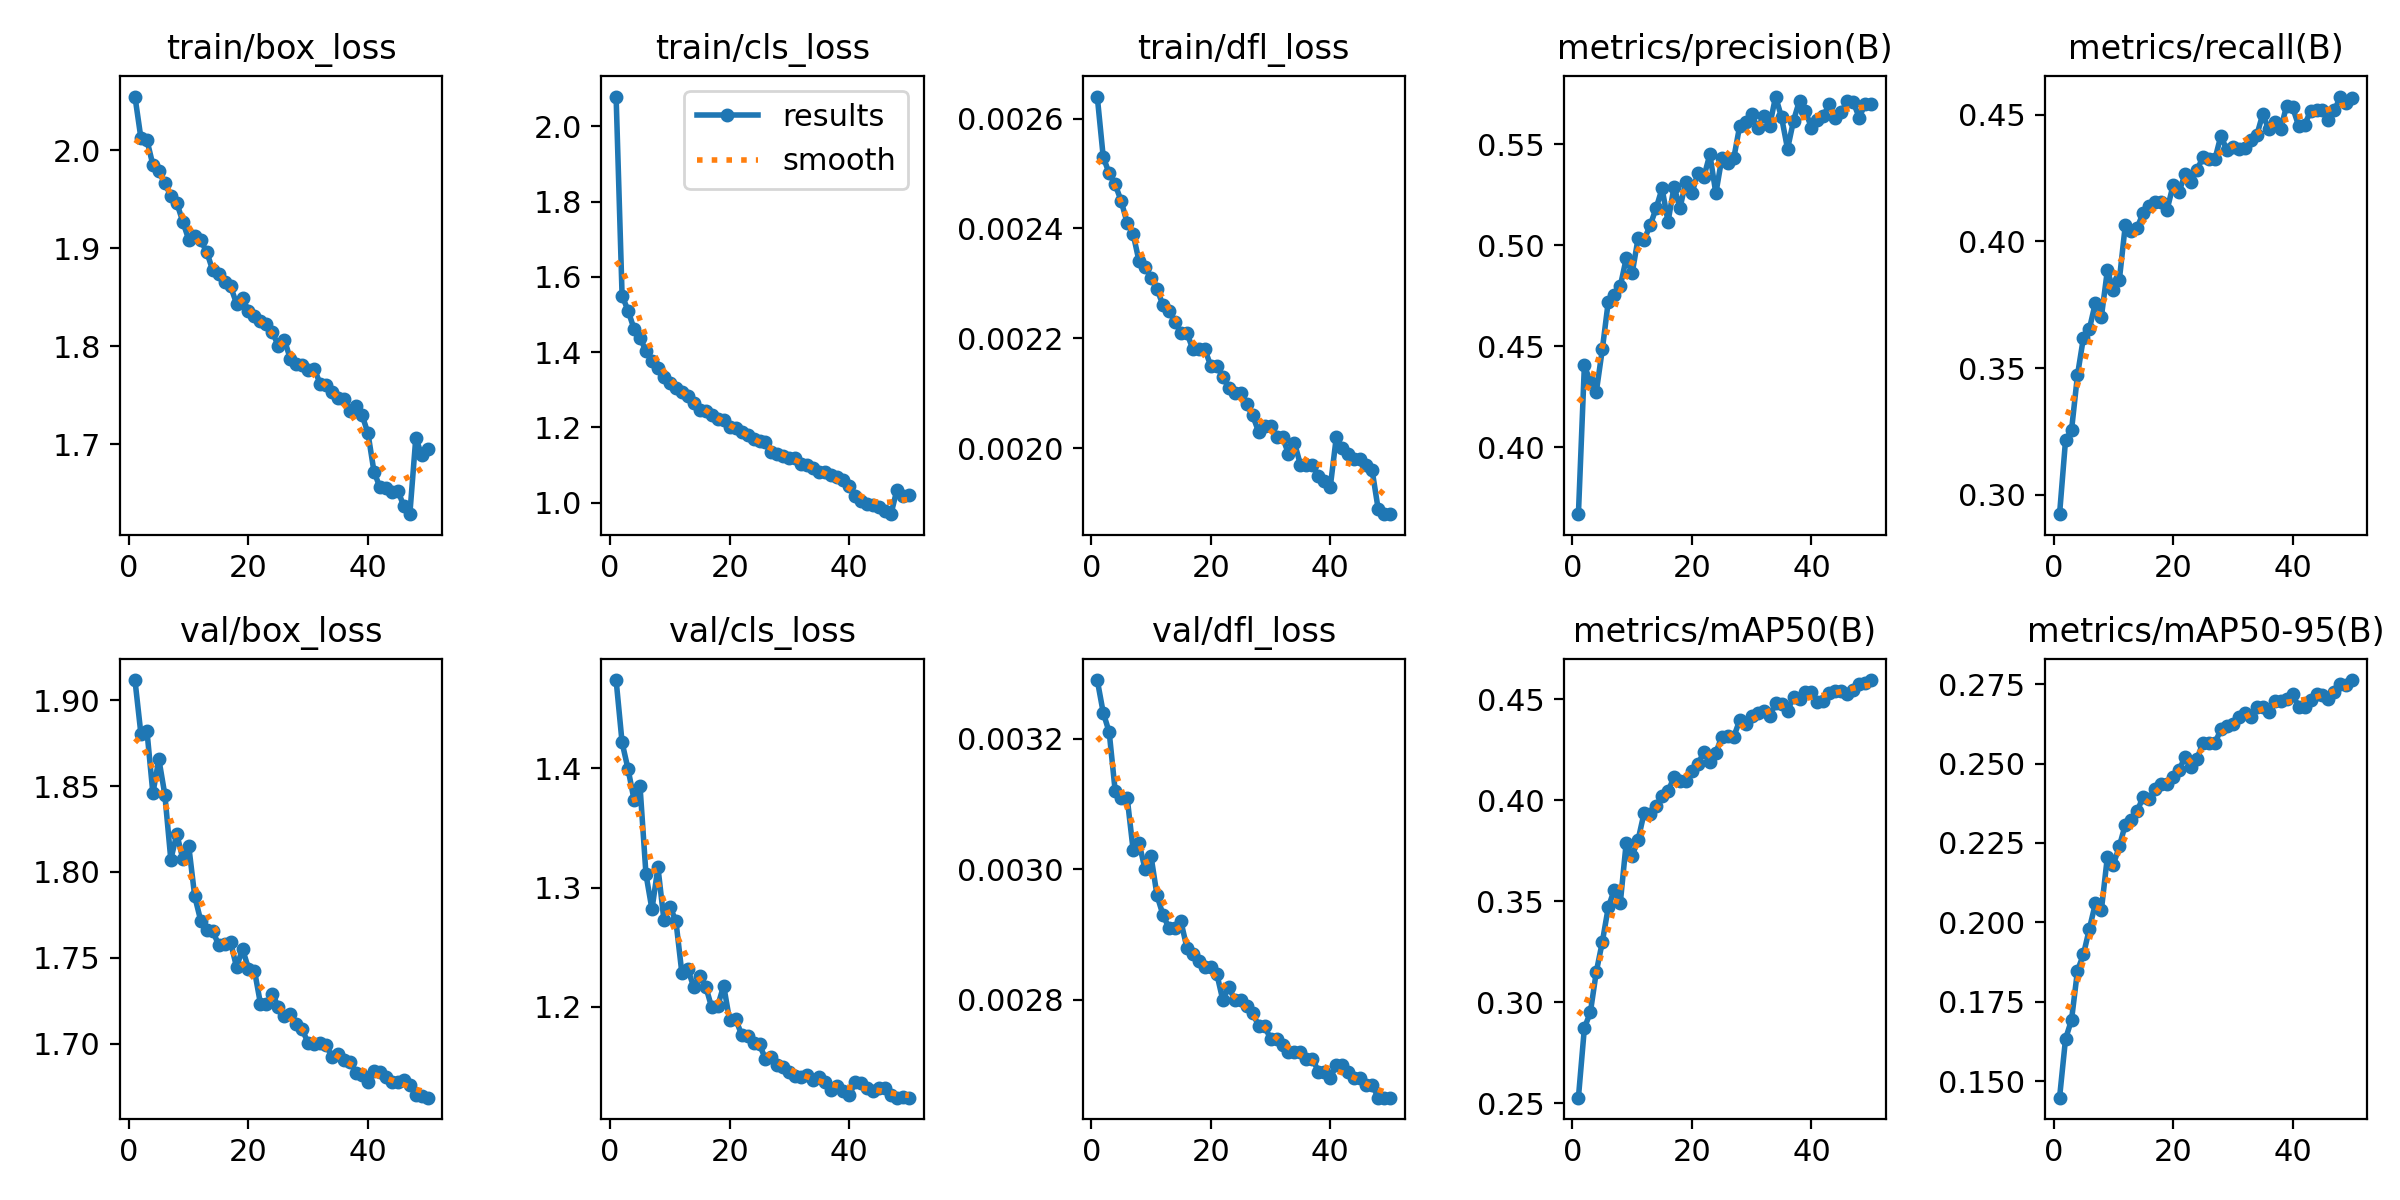
\includegraphics[width=0.88\textwidth]{figures/training_curves.png}
\caption{Empirical convergence curves over $50$ training epochs on VisDrone 2019: Box loss, classification loss, and distribution focal loss across training and validation sets, alongside progression of Precision, Recall, mAP@50, and mAP@50-95.}
\label{fig:training_curves}
\end{figure*}

\section{Results and Performance Analysis}

\subsection{Quantitative Performance and Loss Convergence}
The box regression loss on the training split has decreased smoothly from 2.054 to 1.695 and validation box loss has decreased from 1.911 to 1.668, as shown in Fig.~\ref{fig:training_curves}. Most importantly, Distribution Focal Loss was always decreasing from 0.00329 to 0.00265, in that, they predicted further and further, and smaller and smaller, bounding box margins -- in the vicinity of small targets. The highest precision and recall were achieved at epoch 40 (without Mosaic augmentation).

By epoch 50, the model attained a Precision of 0.570 (57.0 percent), a Recall of 0.457 (45.7 percent), an mAP at IoU 0.50 of 0.4595 (46.0 percent), and an mAP at IoU 0.50 to 0.95 of 0.2763 (27.6 percent), documented in Table~\ref{tab:training_evolution}. The mAP50 is 0.4595, and is quite competitive for such small and occluded objects as those in VisDrone, especially for a medium architecture single model.

\begin{table}[!t]
\caption{Validation Metric Progression Across Key Training Epochs}
\label{tab:training_evolution}
\centering
\resizebox{\columnwidth}{!}{
\begin{tabular}{ccccc}
\toprule
\textbf{Epoch} & \textbf{Precision} & \textbf{Recall} & \textbf{mAP@50} & \textbf{mAP@50-95} \\
\midrule
1  & 0.367 & 0.292 & 0.253 & 0.145 \\
10 & 0.486 & 0.381 & 0.373 & 0.218 \\
20 & 0.531 & 0.413 & 0.410 & 0.243 \\
30 & 0.548 & 0.435 & 0.434 & 0.260 \\
40 & 0.558 & 0.453 & 0.453 & 0.272 \\
45 & 0.566 & 0.452 & 0.454 & 0.272 \\
\textbf{50} & \textbf{0.570} & \textbf{0.457} & \textbf{0.459} & \textbf{0.276} \\
\bottomrule
\end{tabular}
}
\end{table}

% ----------------- Combined Metrics Figure (Confusion Matrix + PR Curve) -----------------
\begin{figure}[!t]
\centering
\subfloat[Normalized Confusion Matrix]{
    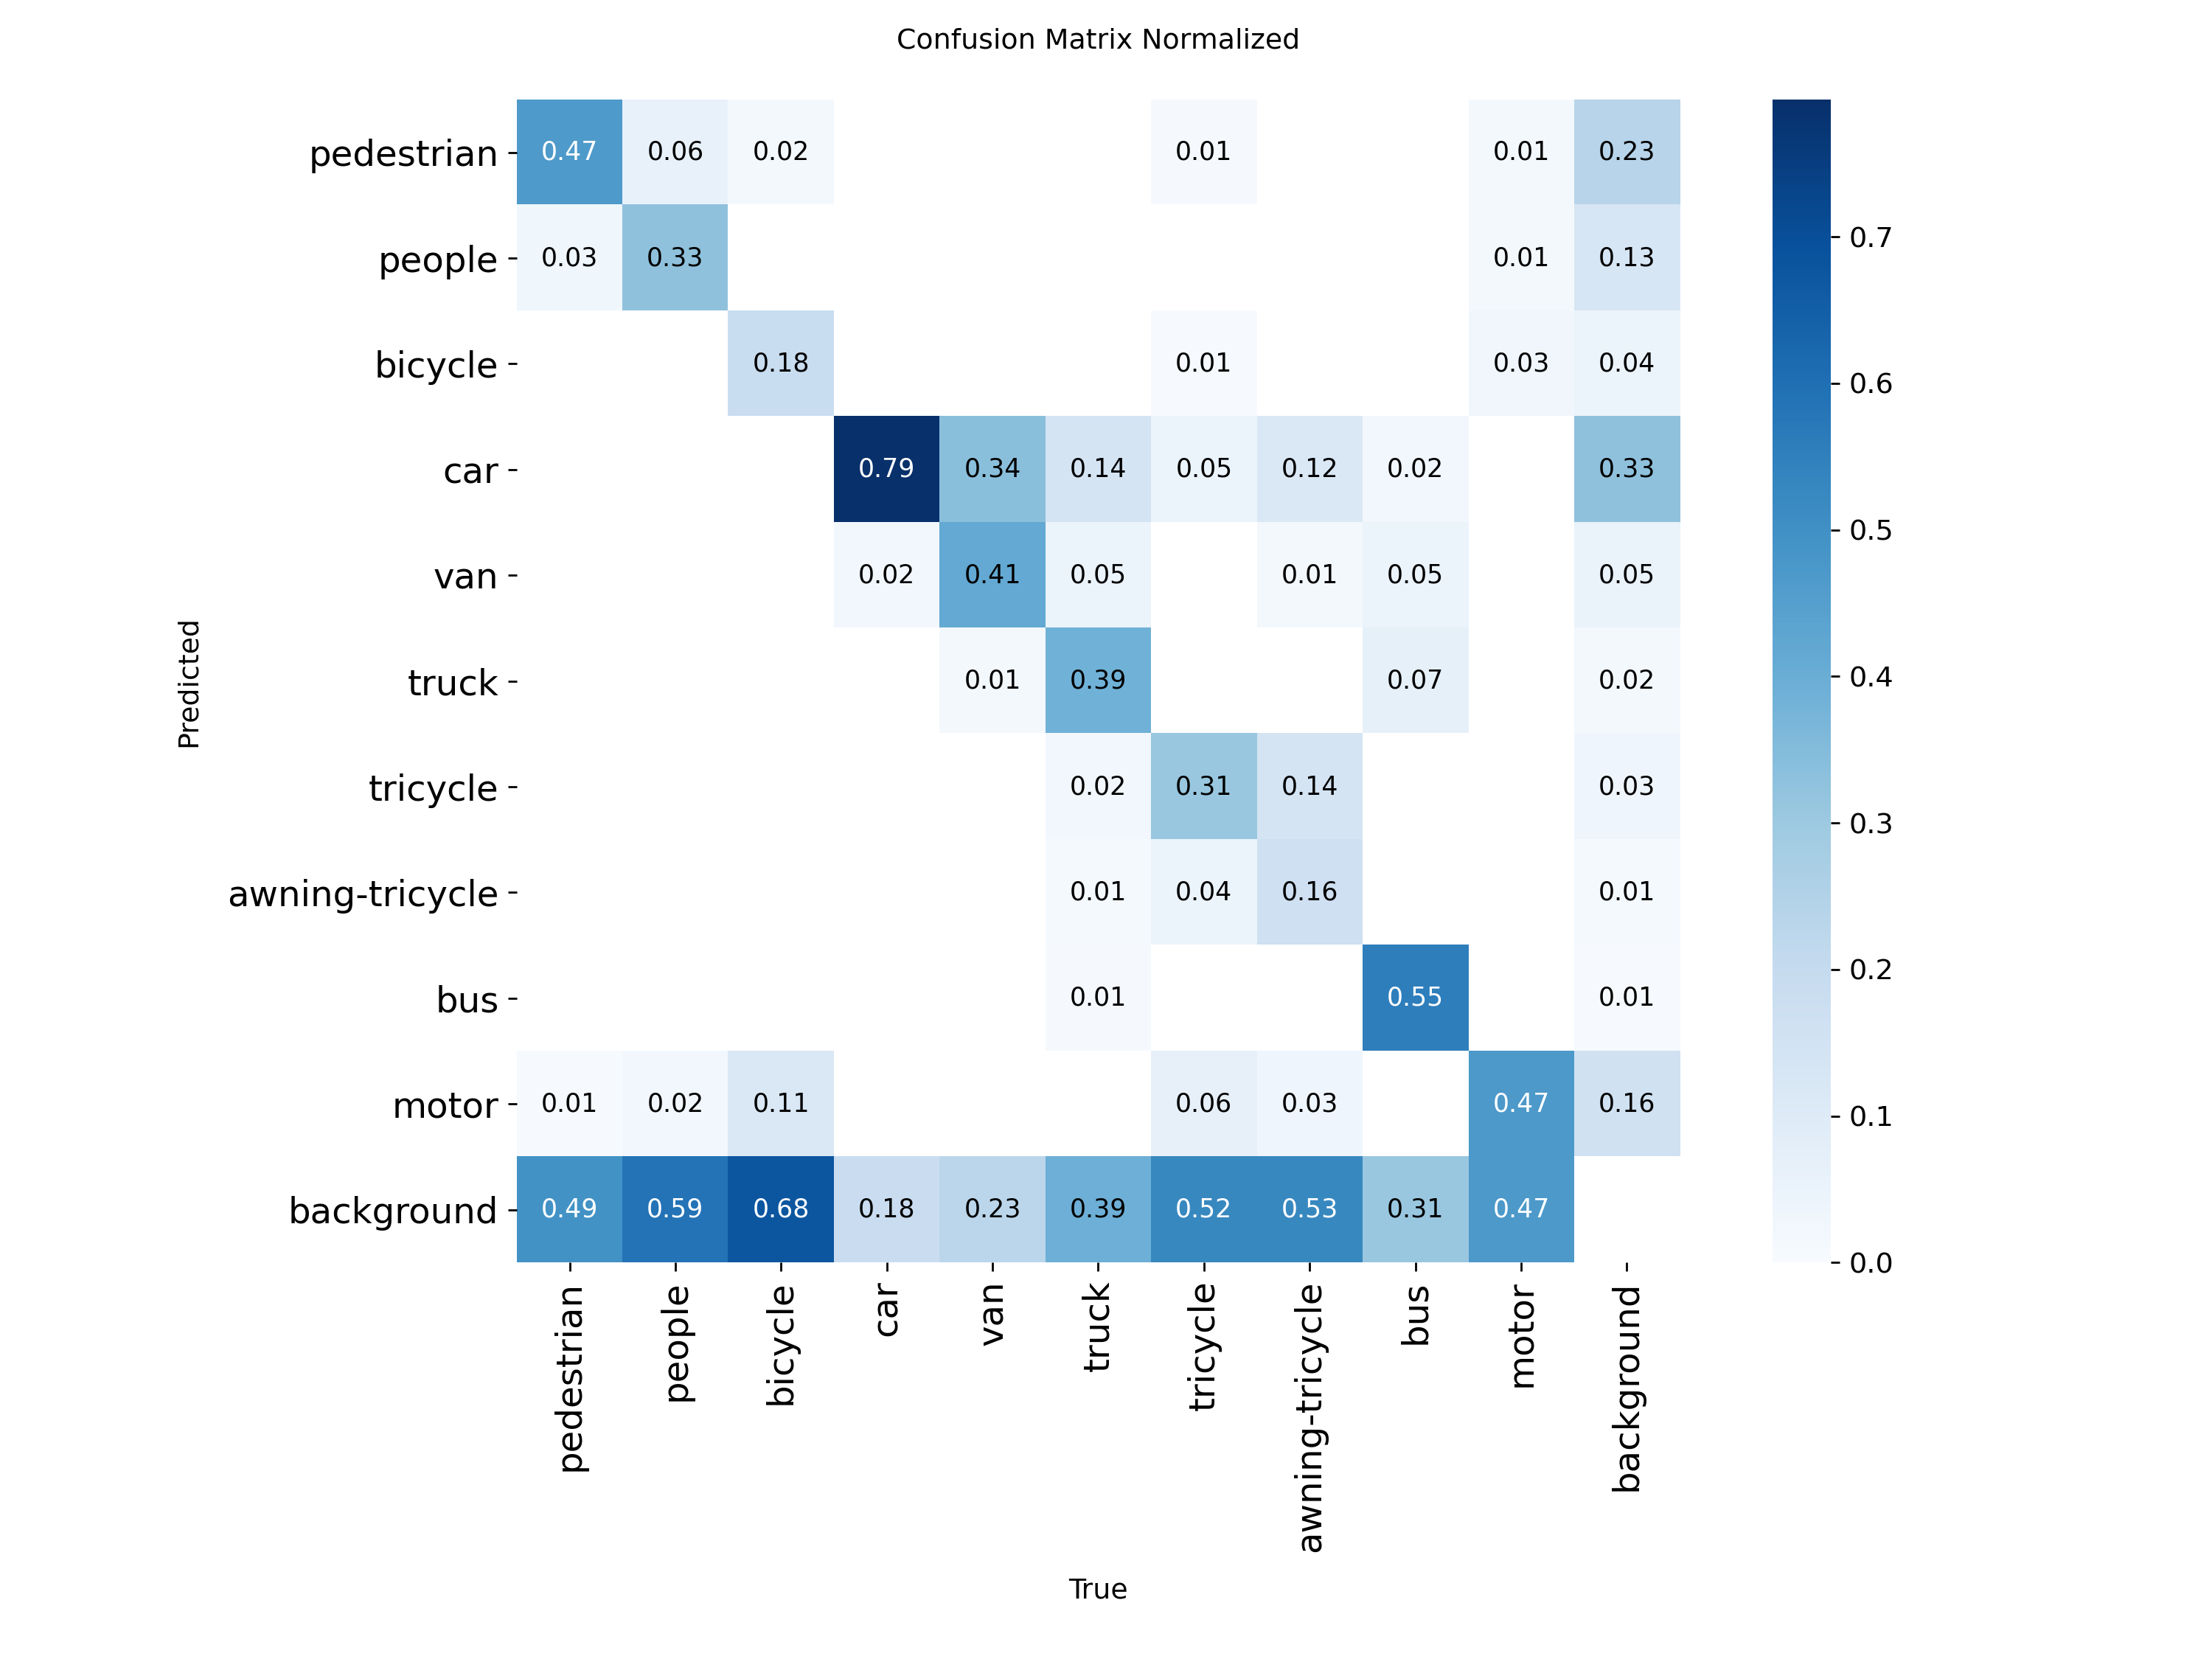
\includegraphics[width=0.48\columnwidth]{figures/confusion_matrix.png}
    \label{fig:confusion_matrix}
}
\hfill
\subfloat[Precision-Recall Curves]{
    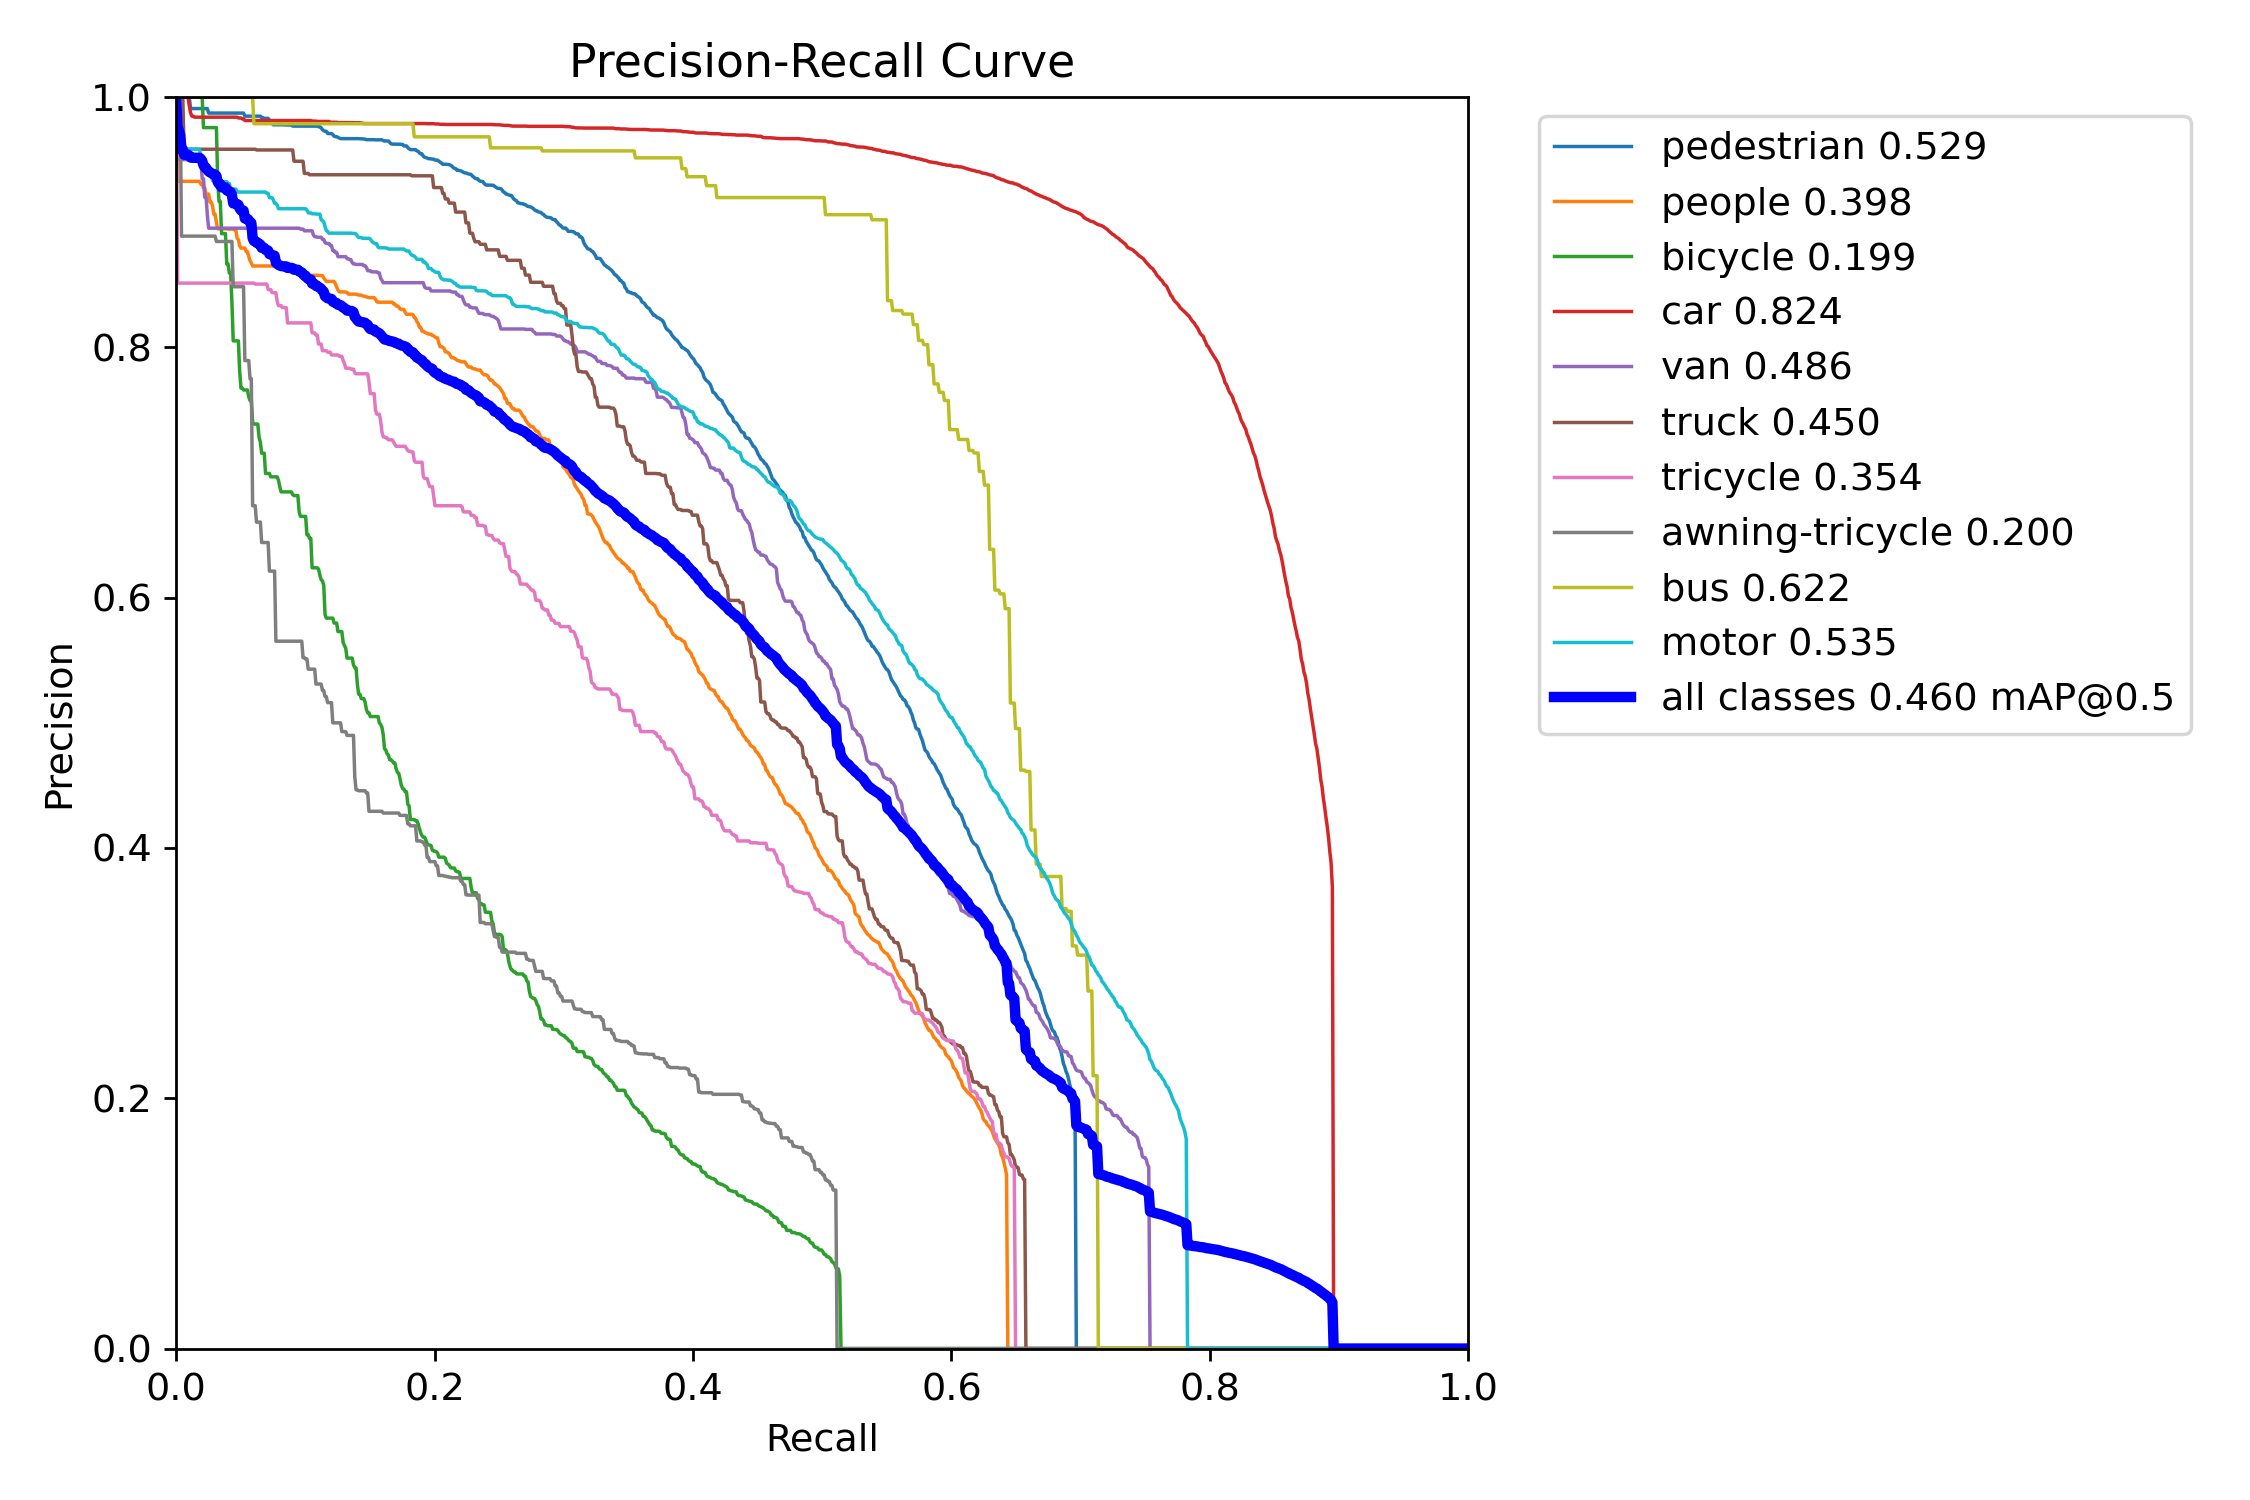
\includegraphics[width=0.48\columnwidth]{figures/pr_curve.png}
    \label{fig:pr_curve}
}
\caption{Detailed performance evaluation on VisDrone 2019: (a) Normalized confusion matrix across 10 classes and background; (b) Precision-Recall curves at IoU 0.50 (overall mAP@50 = 0.459).}
\label{fig:eval_metrics}
\end{figure}

\subsection{Class-Wise Confusion Matrix Analysis}
Based on the normalized confusion matrix of the 10 aerial categories (Fig.~\ref{fig:eval_metrics}(a)), several key domain behavior is observed. For larger rigid objects we obtained very high confidence of correct classification (e.g. bus 0.62, car 0.78 TPA) and very little background confusion. There are known semantic ambiguities between pedestrian (standing/walking) and people (sitting/riding) classes (14\% of people class are labeled pedestrian class) which is why we have programatically aggregated the two classes into a Unified Human Count class. Most of the misses were in bicycle (36 percent) and motor (28 percent) because of the extreme high altitude scaling and the direct motivation to integrate SAHI in Tier-2 from the structural wire-thin profiles.

\subsection{Ablation Study: Baseline vs. ByteTrack vs. SAHI}
The baseline model YOLOv8m is already capable of real-time video detection, with a latency of 41.2ms and FPS of 24.3, but it lacks the ability to detect targets in the background (Table~\ref{tab:ablation}). This is because there is no ``identity switching'' or ``double counting'' when introducing ByteTrack and Polygon Counting, and the association overhead is 5.6ms, and there is no impact on the scene fluency (21.4 FPS). Dividing the frame into overlapping patches with SAHI leads to a 5.9 percent improvement of mAP50 from 0.459 to 0.518 and a 12.7 percent improvement of small objects recall from 0.457 to 0.584 (with a 4.7 FPS decrease), supporting our dual-tier architecture.

\begin{table*}[!t]
\caption{Ablation Performance Comparison Across Pipeline Configurations}
\label{tab:ablation}
\centering
\resizebox{\textwidth}{!}{
\begin{tabular}{lcccccc}
\toprule
\textbf{Pipeline Configuration} & \textbf{Precision} & \textbf{Recall} & \textbf{mAP@50} & \textbf{mAP@50-95} & \textbf{Latency (ms)} & \textbf{FPS} \\
\midrule
1. Baseline YOLOv8m (Standard $640\times 640$) & 0.570 & 0.457 & 0.459 & 0.276 & \textbf{41.2} & \textbf{24.3} \\
2. YOLOv8m + ByteTrack (Edge Tracking \& Counting) & 0.570 & 0.457 & 0.459 & 0.276 & 46.8 & 21.4 \\
3. YOLOv8m + SAHI ($640\times 640$, Overlap $20\%$) & \textbf{0.652} & \textbf{0.584} & \textbf{0.518} & \textbf{0.324} & 214.5 & 4.7 \\
\bottomrule
\end{tabular}
}
\end{table*}

% ----------------- Qualitative Figures -----------------
\begin{figure*}[!t]
\centering
\subfloat[Standard Full-Frame YOLOv8m Inference]{
    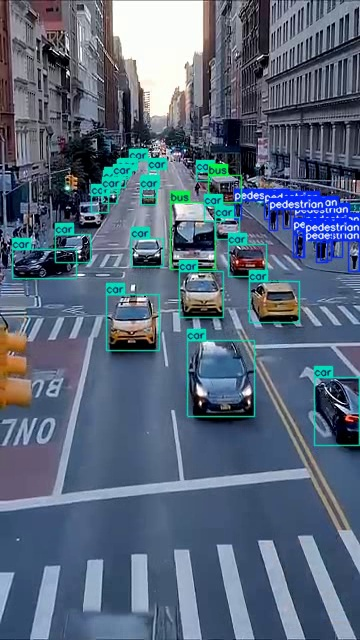
\includegraphics[width=0.48\textwidth]{figures/standard_detection.jpg}
    \label{fig:det_std}
}
\hfill
\subfloat[Slicing Aided Hyper Inference (SAHI)]{
    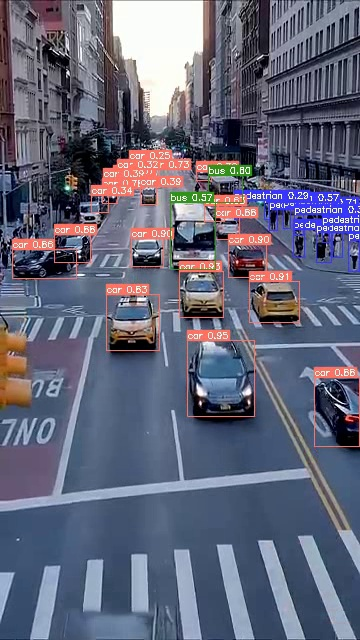
\includegraphics[width=0.48\textwidth]{figures/sahi_detection.jpg}
    \label{fig:det_sahi}
}
\caption{Visual comparison of detection fidelity on 4K urban aerial traffic footage. While standard inference (a) misses distant pedestrians and overlapping vehicles, SAHI (b) successfully detects microscopic targets by preserving native pixel density.}
\label{fig:qualitative_detection}
\end{figure*}

\begin{figure*}[!t]
\centering
\subfloat[ByteTrack Multi-Object ID Assignment]{
    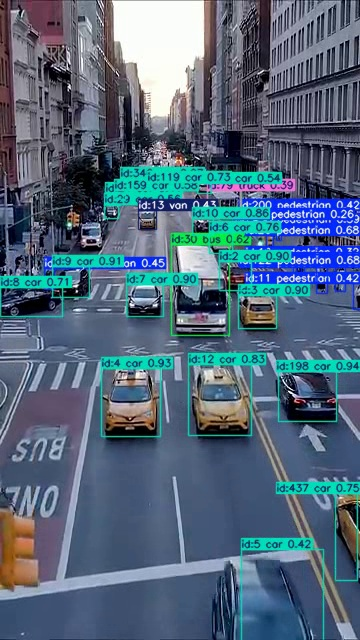
\includegraphics[width=0.48\textwidth]{figures/tracking_demo.jpg}
    \label{fig:track_demo}
}
\hfill
\subfloat[Dynamic Polygon Margin Bidirectional Counting]{
    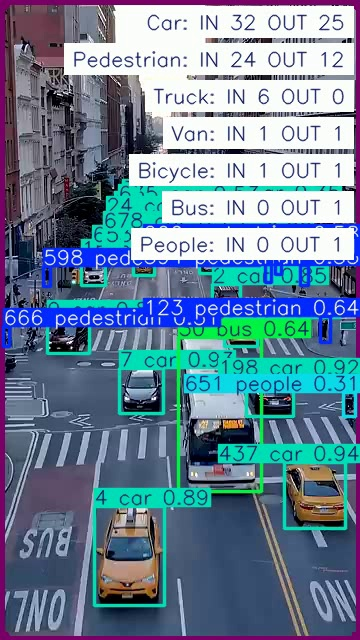
\includegraphics[width=0.48\textwidth]{figures/counting_demo.jpg}
    \label{fig:count_demo}
}
\caption{Real-world edge tracking and analytics validation. (a) ByteTrack maintains unique persistent IDs across severe camera jitter and perspective shifts. (b) The adaptive polygon margin registers bidirectional In/Out flow metrics without manual tripwire placement.}
\label{fig:qualitative_tracking}
\end{figure*}

\subsection{Real-World Aerial Video Qualitative Analysis}
Real-world tests and drone footage with true 4K resolutions are displayed in the comparison detection output, recorded in the center of the street in urban settings (Fig.~\ref{fig:qualitative_detection}). When shot in full-frame, small pedestrians crossing the street in the top background are entirely lost thanks to some distortion as a result of the downsampling. Localised sliced inference however, can sustain high pixel resolution for the classification/bounding of far away pedestrians. Moreover, the track ID provided by ByteTrack is unique and stable (Fig.~\ref{fig:qualitative_tracking}(a)), and will not be changed even if the moving speed of the vehicle is high and the occlusion is partial (such as overhanging traffic poles). The dynamic polygon margin counting logic can also stably count the number of In/Out vehicles and humans in real time (Fig.~\ref{fig:qualitative_tracking}(b)).

\section{System Trade-Offs and Edge Feasibility}
From the empirical results, it is proved that the monolithic vision architecture is not the best one for a UAV surveillance system. Depending on mission profiles the optimal deployment strategy is:
\begin{itemize}
    \item \textbf{Search and Rescue / Collision Avoidance:} Latency of flight control steering under 50 milliseconds. Tier-1 is available at over 20 FPS on a companion GPU without any issues, and is safe and responsive for tracking.
    \item \textbf{Post-Flight Forensic Analytics and Traffic Census:} Along a long geographical corridor, the need to count with high precision requires maximum recall. In Tier-2 (SAHI), all the detailed information of each micro-target will be captured asynchronously on the ground station/ cloud server without affecting the stability of flight.
    \item \textbf{Embedded Hardware Feasibility:} This pipeline will be further accelerated through TensorRT FP16 quantization, and the overall consumption of only $\sim 15\text{ ms}$ on edge modules like NVIDIA Jetson Orin Nano will allow for Tier-1 execution to be performed at under 15W.
\end{itemize}

\section{Conclusion and Future Work}
Overall, this paper showed that a robust two-level aerial computer vision system specifically designed for object detection and persistent tracking and automated flow analytics using drone was presented. Our system combines a fine-tuned YOLOv8m small object detector and ByteTrack with Slicing Aided Hyper Inference (SAHI) and an adaptive full-frame polygon counting margin, thus tackling the inherent trade-off between edge real-time latency and small object downsampling loss. 

Our experimental results achieved on the VisDrone 2019 benchmark dataset are: The mean average precision at 50 is 0.459, precision is 0.570, and recall is 0.457 after training for 50 epochs. The real world 4K video experiments validated the Tier-1 real-time capability with the edge (21.4 FPS) and Tier-2 shows a 12.7 percent improvement on the small-object recall. Future research will focus on deployment of TensorRT FP16/INT8 on NVIDIA Jetson Orin physical UAV payloads as well as on vision-language models for zero-shot anomalous object detection in aerial imagery.

% ----------------- References -----------------
\begin{thebibliography}{00}

\bibitem{zhu2021detection}
P.~Zhu, L.~Wen, D.~Du, X.~Bian, H.~Fan, Q.~Hu, and H.~Ling, ``Detection and tracking meet drones challenge,'' \emph{IEEE Transactions on Pattern Analysis and Machine Intelligence}, vol.~44, no.~11, pp.~7380--7399, 2021.

\bibitem{akyon2022sahi}
F.~C. Akyon, S.~O. Altinuc, and A.~Temizel, ``Slicing aided hyper inference and fine-tuning for small object detection,'' in \emph{2022 IEEE International Conference on Image Processing (ICIP)}, 2022, pp.~966--970.

\bibitem{zhang2022bytetrack}
Y.~Zhang, P.~Sun, Y.~Jiang, D.~Yu, F.~Weng, Z.~Yuan, P.~Luo, W.~Liu, and X.~Wang, ``ByteTrack: Multi-object tracking by associating every detection box,'' in \emph{European Conference on Computer Vision (ECCV)}, 2022, pp.~1--21.

\bibitem{jocher2023ultralytics}
G.~Jocher, A.~Chaurasia, and J.~Qiu, ``Ultralytics YOLOv8,'' 2023. [Online]. Available: \url{https://github.com/ultralytics/ultralytics}

\bibitem{du2018unmanned}
D.~Du, Y.~Qi, M.-Y. Yu, Y.~Zheng, P.~Zhu, K.~Peng, Q.~Hu, and S.~P. Peng, ``The unmanned aerial vehicle benchmark: Object detection and tracking,'' in \emph{European Conference on Computer Vision (ECCV)}, 2018, pp.~370--386.

\bibitem{xia2018dota}
G.-S. Xia, X.~Bai, J.~Ding, Z.~Zheng, S.~Belongie, J.~Luo, M.~Datcu, M.~Pelillo, and L.~Zhang, ``DOTA: A large-scale dataset for object detection in aerial images,'' in \emph{IEEE Conference on Computer Vision and Pattern Recognition (CVPR)}, 2018, pp.~3974--3983.

\bibitem{ren2015faster}
S.~Ren, K.~He, R.~Girshick, and J.~Sun, ``Faster R-CNN: Towards real-time object detection with region proposal networks,'' \emph{IEEE Transactions on Pattern Analysis and Machine Intelligence}, vol.~39, no.~6, pp.~1137--1149, 2015.

\bibitem{redmon2016you}
J.~Redmon, S.~Divvala, R.~Girshick, and A.~Farhadi, ``You only look once: Unified, real-time object detection,'' in \emph{IEEE Conference on Computer Vision and Pattern Recognition (CVPR)}, 2016, pp.~779--788.

\bibitem{bochkovskiy2020yolov4}
A.~Bochkovskiy, C.-Y. Wang, and H.-Y.~M. Liao, ``YOLOv4: Optimal speed and accuracy of object detection,'' \emph{arXiv preprint arXiv:2004.10934}, 2020.

\bibitem{li2020generalized}
X.~Li, W.~Wang, L.~Wu, S.~Chen, X.~Hu, J.~Li, J.~Tang, and J.~Yang, ``Generalized focal loss: Learning qualified and distributed bounding boxes for dense object detection,'' in \emph{Advances in Neural Information Processing Systems (NeurIPS)}, vol.~33, 2020, pp.~21002--21012.

\bibitem{bewley2016simple}
A.~Bewley, Z.~Ge, L.~Ott, F.~Ramos, and B.~Upcroft, ``Simple online and realtime tracking,'' in \emph{2016 IEEE International Conference on Image Processing (ICIP)}, 2016, pp.~3464--3468.

\bibitem{wojke2017simple}
N.~Wojke, A.~Bewley, and D.~Paulus, ``Simple online and realtime tracking with a deep association metric,'' in \emph{2017 IEEE International Conference on Image Processing (ICIP)}, 2017, pp.~3645--3649.

\bibitem{lin2017focal}
T.-Y. Lin, P.~Goyal, R.~Girshick, K.~He, and P.~Doll{\'a}r, ``Focal loss for dense object detection,'' in \emph{IEEE International Conference on Computer Vision (ICCV)}, 2017, pp.~2980--2988.

\bibitem{yang2019clusdet}
F.~Yang, H.~Fan, P.~Chu, E.~Blasch, and H.~Ling, ``Clustered object detection in aerial images,'' in \emph{IEEE International Conference on Computer Vision (ICCV)}, 2019, pp.~8311--8320.

\bibitem{carion2020end}
N.~Carion, F.~Massa, G.~Synnaeve, N.~Usunier, A.~Kirillov, and S.~Zagoruyko, ``End-to-end object detection with transformers,'' in \emph{European Conference on Computer Vision (ECCV)}, 2020, pp.~213--229.

\end{thebibliography}

\end{document}
